\section{(Alternate) General Search Box}
\label{sec:general_search}

A general search text box is available to query the entire collection of
manually curated information in ELM DB. This search field can be found at the
top of almost all pages on the ELM website (for example in Fig.
\ref{fig:general_search_TP53_instances}). This search is a full-text
search across multiple selected data sources in the database, including
protein and ELM class. 

%
% Subsection: Necessary Resources
%
\subsection{Necessary Resources}
\subsubsection{Software \& Hardware}
%A modern browser such as Firefox, Chrome, or Safari. ELM is best viewed
on a laptop or desktop computer, although tablets and smartphones will
also work.


%
% Subsection: General search 
%
\subsection{Using the General Search}
\label{subsec:general_search_using}
A modern browser such as Firefox, Chrome, or Safari. ELM is best viewed
on a laptop or desktop computer, although tablets and smartphones will
also work.


\begin{enumerate}

\begin{figure}[h!]
	\centering
	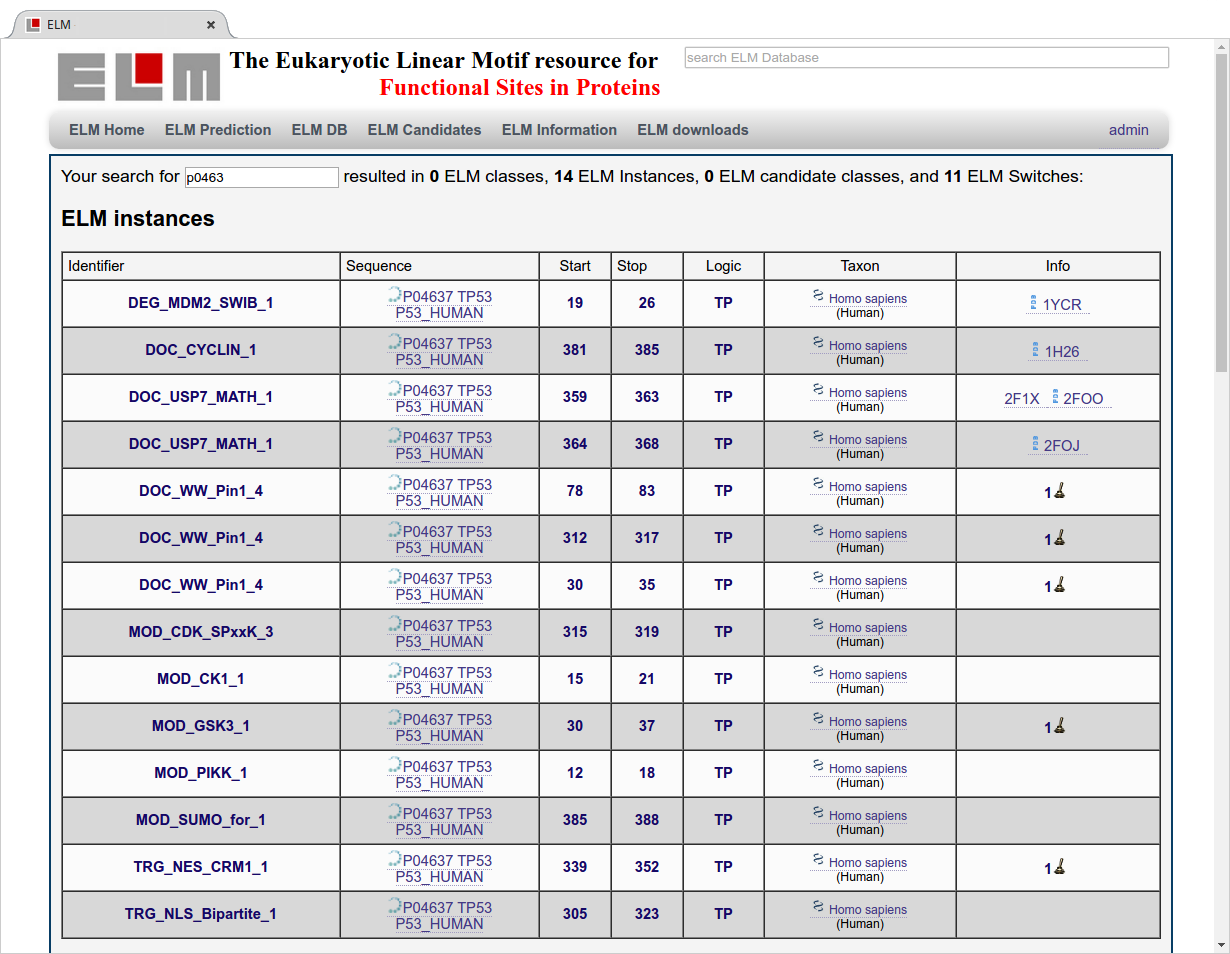
\includegraphics[width=\textwidth]{Figures/general_search/P04637_instances.png} 
	\caption{
		The instances retrieved when performing a general search for
		\uniprot{P53\_Human} using its Uniprot identifier ``P04637''.
	}
	\label{fig:general_search_P04637_instances}
\end{figure}

\begin{figure}[h!]
	\centering
	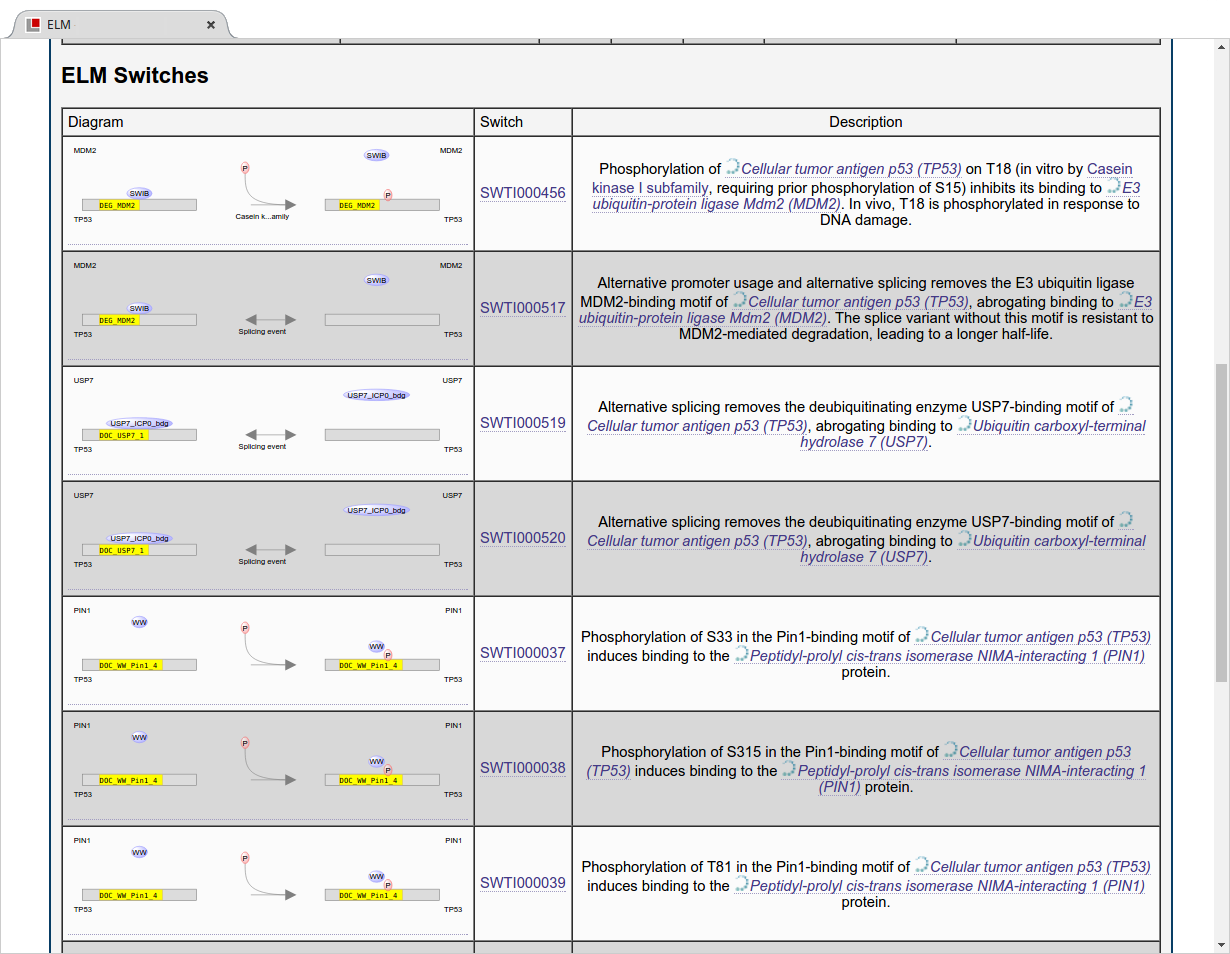
\includegraphics[width=\textwidth]{Figures/general_search/P04637_switches.png} 
	\caption{
		The switches found when performing a general search for
		\uniprot{P53\_Human} using its Uniprot identifier ``P04637'',
	}
	\label{fig:general_search_P04637_switches}
\end{figure}


\item Use the general search field (on the top of the page) to do a general
	seach for P53 using its Uniprot identifier by typing ``P04637'' in the
	search field and hitting ``Enter''. This will search
	across instances, motif classes and switches to find any matches to the
	search query ``P04637''. 
	The results are grouped into matching instances
	(Fig. \ref{fig:general_search_P04637_instances})
	candidate classes and switches
	(Fig. \ref{fig:general_search_P04637_switches}).
	As there are no classes with ``P04637'' in the name, no classes are
	returned with this query.

	\sdesc{
		The ``candidate classes'' are a separate part of ELM, where
		users can propose novel classes to be annotated. Although these
		are returned by the general search, we would advise users not
		to use this data, as it is still pending curation.
	}

\begin{figure}[h!]
	\centering
	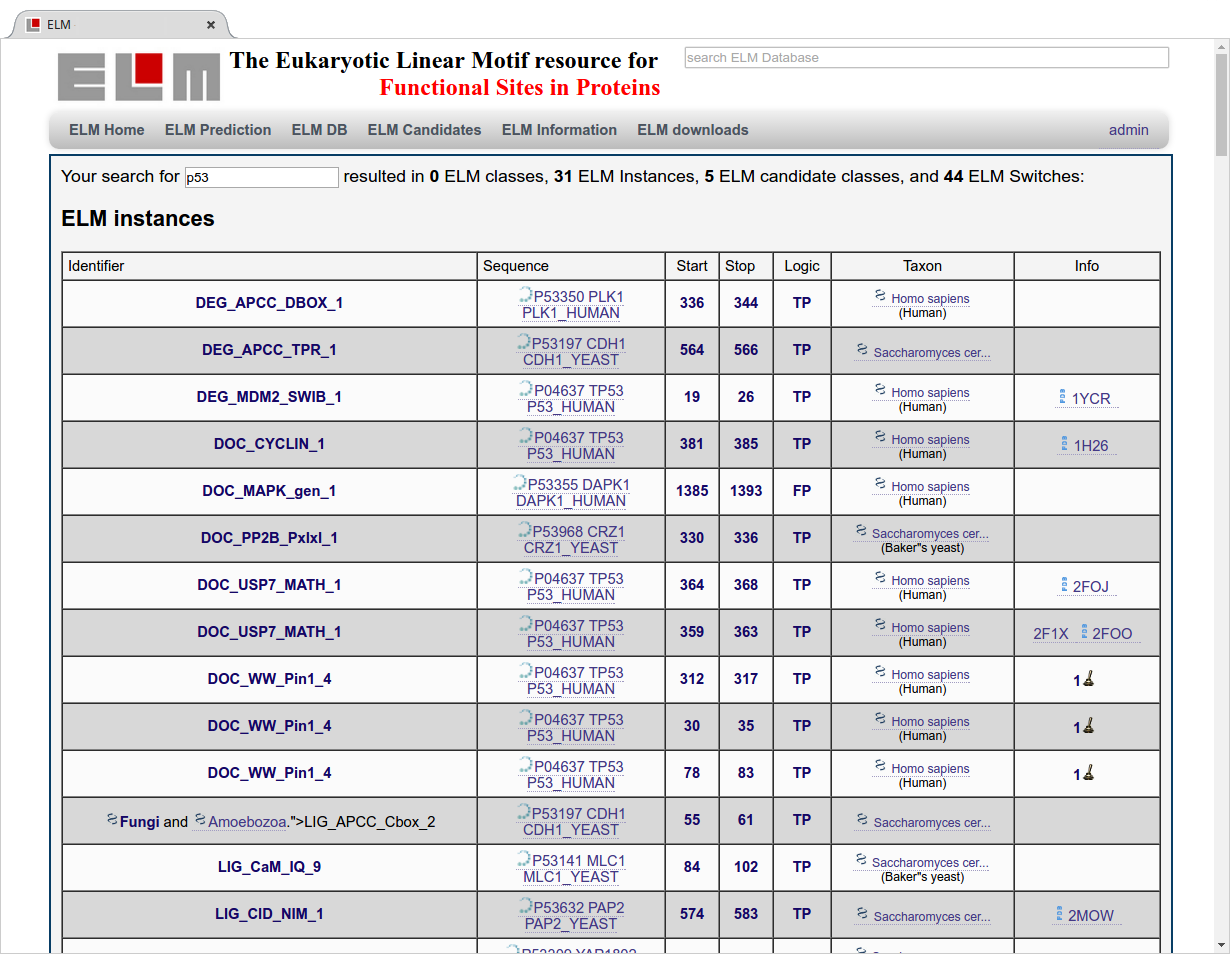
\includegraphics[width=\textwidth]{Figures/general_search/TP53_instances.png} 
	\caption{
		The results retrieved when performing a general search for
		\uniprot{P53\_Human} using the query ``p53''.
	}
	\label{fig:general_search_TP53_instances}
\end{figure}

\item Perform a search using the keyword ``p53'' in the general search field
	instead of its Uniprot identifier ``P04637''.
	The set of results retrieved using this term as search query
	(Fig. \ref{fig:general_search_TP53_instances})
	in this case are different, returning 31 instances and 44
	switches (instead of 14 and 11). The reason for this is that the
	phrase ``P53'' also matches the Uniprot identifier of
	\uniprot{CDH1\_YEAST} (P53197). This is important to keep in mind when
	using the general search field.

\end{enumerate}
